\documentclass{beamer}
\usepackage[latin1]{inputenc}
\usepackage{amsmath}
\usepackage{graphicx}
\usepackage{multimedia}
\usepackage{caption}
\usetheme{default}
\usecolortheme{default}
\definecolor{darkred}{RGB}{24,0,0}
\setbeamercolor{title}{fg=red}
%\setbeamercolor{frametitle}{fg=black}
\setbeamertemplate{blocks}[rounded][shadow=true]
\setbeamertemplate{itemize items}[square]
\usefonttheme{serif}
\title{\textit{\textbf{\'Atomo de Hidr\'ogeno relativista en el formalismo de Dirac.}}}
\author{Juan Nicol\'as Garavito Camargo \\ Juan David Orjuela Zu\~niga}
\institute{Universidad de los Andes, Bogot\'a, Colombia}
\date{May 27, 2015}
\begin{document}

\begin{frame}
\titlepage
\author
\institute
\begin{figure}
%\rule{1.28cm}{0.72cm}

\includegraphics[scale=0.35]{Figures/logo.jpeg}
\end{figure}
\end{frame}


\begin{frame}
\begin{figure}
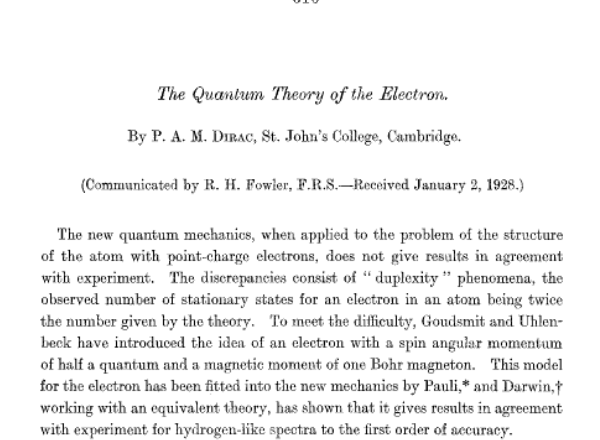
\includegraphics[scale=0.4]{Figures/dirac1928.png}
\end{figure}
\end{frame}


\begin{frame}
\begin{figure}
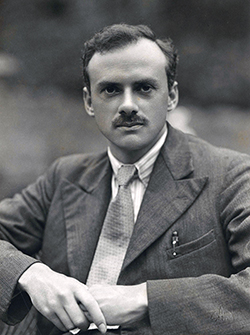
\includegraphics[scale=0.5]{Figures/dirac.jpg}
\caption{P.A.M. Dirac}
\end{figure}
\end{frame}

\begin{frame}{\textit{\textbf{La ecuaci\'on de Dirac se deduce a partir de argumentos de simetr\'ia provenientes de la relatividad especial}}}
\[
\dfrac{1}{c}\dfrac{\partial \psi_i(\mathbf{r},t)}{\partial t} =
- \sum \limits_{k=x,y,z} \sum \limits_{n=1}^{N}\alpha^k_{i,n} \dfrac{\partial \psi_n}{\partial k} -
\dfrac{imc}{\hbar}\sum \limits_{n=1}^{N}\beta_{i,n}\psi_n(\mathbf{r}, t)
\]
\end{frame}

\begin{frame}{\textit{\textbf{Las matrices}} $\widetilde{\alpha}$ \textit{\textbf{y}} $\widetilde{\beta}$ \textit{\textbf{se definen:}}}
\begin{equation}
E\phi(\mathbf{r},t) =
(c\widetilde{\alpha}\cdot \hat{\mathbf{p}} + \widetilde{\beta}mc^2 + V(r))\phi(\mathbf{r})
\end{equation}

\begin{equation}
\widetilde{\alpha_i}=
\begin{pmatrix}
0 & \widetilde{\sigma}_i\\
\widetilde{\sigma}_i & 0 \\
\end{pmatrix}
\end{equation}

\begin{equation}
\widetilde{\beta}=
\begin{pmatrix}
\widetilde{\mathbf{I}}_2 & 0\\
0 & -\widetilde{\mathbf{I}}_2 \\
\end{pmatrix}
\end{equation}

\end{frame}

\begin{frame}{\textit{\textbf{\'Atomo de Hidrogeno realtivista y con spin}}}

\[
(c \widetilde{\alpha} \cdot \hat{p} + \widetilde{\beta} m c^2 + V(r) ) \phi(r) = E \phi (r)
\]

\begin{equation}
V(r) = \dfrac{Ze^2}{4\pi\epsilon_0 r^2}
\end{equation}
\end{frame}

\begin{frame}{\textit{\textbf{Transformaci\'on a coordenadas esfericas}}}
\begin{equation}\label{eq:alphap}
\widetilde{\alpha} \cdot \hat{\mathbf{p}} = -i \hbar \widetilde{\alpha} \cdot \nabla
\end{equation}

\begin{equation}\label{eq:nabla}
\mathbf{\nabla} =  \hat{\mathbf{r}}(\dfrac{\partial}{\partial r}) - \dfrac{i}{\hbar}\dfrac{\hat{\mathbf{r}}}{r} \times \mathbf{L}
\end{equation}

Por lo tanto (\ref{eq:alphap}) se puede escribir en t\'erminos de (\ref{eq:nabla}) como:

\begin{equation}\label{eq:alphap2}
\widetilde{\alpha}\cdot \mathbf{\hat{p}} = -i\hbar \widetilde({\alpha}\cdot \hat{\mathbf{r}}(\dfrac{\partial}{\partial r}) - 
\dfrac{i}{\hbar}\widetilde{\alpha}\cdot \dfrac{\hat{\mathbf{r}}}{r} \times \mathbf{L})
\end{equation}
\end{frame}

\begin{frame}{\textbf{\textit{Definici\'on del n\'umero cuantico}} $\kappa$}
\begin{equation}
\widetilde{\hat{K}} = \widetilde{\hat{L}}\cdot \widetilde{\sigma} + \hbar
\end{equation}

Con autovalor $-\hbar \kappa$ y donde $\kappa$ puede tomar los siguientes
valores:

\[ \kappa = 
\begin{cases}
-l - 1 \rightarrow j = l + 1/2  \\
l \rightarrow j = l - 1/2 \\ 
\end{cases}
\]  

\end{frame}

\begin{frame}{\textit{\textbf{Ecuaci\'on de Dirac en coordenadas esfericas}}}
\begin{equation}\label{alphap4}
\widetilde{\alpha} \cdot \mathbf{\hat{p}} = -i\hbar \widetilde{\alpha}\cdot \hat{\mathbf{r}}\partial_r + \dfrac{i}{|\mathbf{r}|} \widetilde{\alpha_r}(\widetilde{\beta}\hat{K}-\hbar)
\end{equation}

\begin{equation}\label{eq:radialdirac}
\left (ic\widetilde{\gamma_5}\widetilde{\sigma_r} \left (\hbar \partial_r + \dfrac{\hbar}{r} -  \dfrac{\widetilde{\beta}\hat{K}}{r}\right )  + \widetilde{\beta} m c^2 + V(r) \right ) \phi(r) = E \phi (r)
\end{equation}

\end{frame}

\begin{frame}
\begin{equation}\label{eq:funciondeonda}
\phi^{m_j}_{\kappa} (\vec{r} ) = \left( \substack{g_{\kappa}(r)\chi^{m_j}_\kappa (\hat{r}) \\ if_\kappa(r)\chi^{m_j}_{-\kappa} (\hat{r}) } \right) 
\end{equation}
\begin{equation}
-c \hbar  \left( \frac{\partial}{\partial r}+\frac{1}{r}+\frac{\kappa}{r} \right) g_{\kappa}(r)\chi^{m_j}_{-\kappa} +(E-V(r)+mc^2)f_{\kappa}(r)\chi^{m_j}_{-\kappa}
\end{equation}


\begin{equation}
c \hbar  \left( \frac{\partial}{\partial r}+\frac{1}{r}+\frac{\kappa}{r} \right) f_{\kappa}(r)\chi^{m_j}_{\kappa} +(E-V(r)-mc^2)g_{\kappa}(r)\chi^{m_j}_{\kappa}
\end{equation}

\end{frame}

\begin{frame}{\textit{\textbf{Separaci\'on de variables}}}
\begin{equation}
\frac{\partial g_{\kappa}(r)}{\partial r} =\frac{\kappa+1}{r}g_{\kappa}(r)+\frac{1}{c\hbar}(E-V(r)+mc^2)f_{\kappa}(r)
\end{equation}

\begin{equation}
\frac{\partial f_{\kappa}(r)}{\partial r} =\frac{\kappa-1}{r}f_{\kappa}(r)-\frac{1}{c\hbar}(E-V(r)-mc^2)g_{\kappa}(r)
\end{equation}
\end{frame}

\begin{frame}{\textit{\textbf{Cambiando de variables}}}

\[
u_{\kappa} = r g_{\kappa}(r), \nu_{\kappa} = r f_{\kappa}(r)
\]

\begin{equation}\label{eq:Hrad1}
\dfrac{\partial u_{\kappa}(r)}{\partial r} =-\dfrac{\kappa}{r}u_{\kappa}(r)+\left ( Wc+\dfrac{\xi}{r}+K_C \right ) v_{\kappa}(r)
\end{equation}

\begin{equation}\label{eq:Hrad2}
\dfrac{\partial v_{\kappa}(r)}{\partial r} =\dfrac{\kappa}{r}v_{\kappa}(r)+
\left ( W_C + \dfrac{\xi}{r} - k_C \right )u_{\kappa}(r)
\end{equation}

En donde $k_C = mc/\hbar$ se denomina el vector de onda de Compton y 
$W_C = E / c\hbar$.
\end{frame}

\begin{frame}
\begin{equation}\label{eq:cdv}
u_{\kappa}(r) = (k_C + W_C)^{1/2} e^{-\lambda r}(\phi_1 + \phi_2)
\end{equation}

\begin{equation}
\nu_{\kappa}(r) = (k_C - W_C )^{1/2} e^{-\lambda r} (\phi_1 - \phi_2)
\end{equation}

En donde $\lambda = (k_C^2 - W_C^2)^{1/2}$
\end{frame}



\begin{frame}
Haciendo el cambio de variable de $r$ a una variable adimensional $\rho = 2 \lambda r$
se obtiene:

\begin{equation}\label{eq:sol1}
\dfrac{\partial \phi_1}{\partial \rho} = \left( 1-\dfrac{\xi W_C}{\lambda  \rho} \right) 
\phi_1 - \left( \dfrac{\kappa}{\rho} + \dfrac{\xi k_C}{\lambda \rho}  \right)\phi_2
\end{equation}

\begin{equation}\label{eq:sol2}
\dfrac{\partial \phi_2}{\partial \rho} = \dfrac{\xi W_C}{\lambda  \rho} \phi_2 
+ \left( -\dfrac{\kappa}{\rho} + \dfrac{\xi k_C}{\lambda \rho}  \right)\phi_1
\end{equation}
\end{frame}

\begin{frame}
\begin{equation}\label{eq:phi1}
\phi_1(\rho) = \rho^s \sum \limits_{m=0}^{\infty} a_m \rho^m
\end{equation}


\begin{equation} \label{eq:phi2}
\phi_2(\rho) = \rho^s \sum \limits_{m=0}^{\infty} b_m \rho^m
\end{equation}

\end{frame}

\begin{frame}
\begin{equation}\label{eq:sol1}
\phi_1(\rho) = 	\rho^s a_0 M(1-n',2s+1,\rho)
\end{equation}

\begin{equation}\label{eq:sol2}
\phi_2(\rho) = \rho^s b_0 M(-n',2s+1,\rho) = \rho^s \dfrac{\kappa - \xi kc / \lambda}{n'} a_0 M(-n',2s+1,\rho)
\end{equation}
\end{frame}

\begin{frame}{condiciones de frontera}
\begin{figure}[H]
\centering
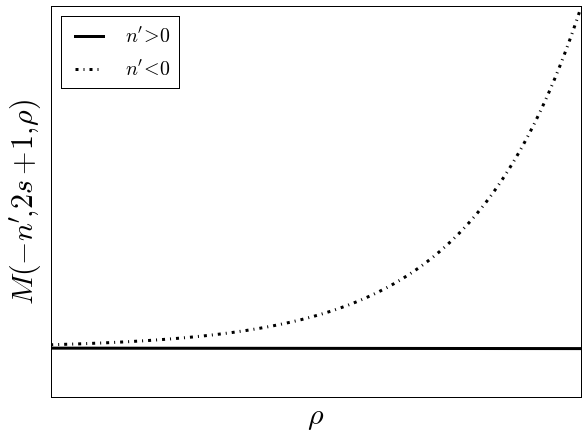
\includegraphics[scale=0.4]{../doc/hypgeo.png}
\caption*{Comportamiento asint\'otico de la funci\'on hipergeom\'etrica.}
\label{fig:hypgeo}
\end{figure}  
\end{frame}

\begin{frame}

\begin{equation}
\begin{split}
f_{\kappa}(r)=2\lambda (k_C -W_C)^{1/2}e^{-\lambda r}(2\lambda r)^{s-1}a_0 \times \\
\left( M(1-n',2s+1,2\lambda r) - \frac{\kappa-\xi k_C /\lambda}{n'} M(-n',2s+1,2\lambda r) \right)
\end{split}
\end{equation}

\begin{equation}
\begin{split}
g_{\kappa}(r)=2\lambda (k_C +W_C)^{1/2}e^{-\lambda r}(2\lambda r)^{s-1}a_0 \times \\
\left( M(1-n',2s+1,2\lambda r) - \frac{\kappa-\xi k_C /\lambda}{n'} M(-n',2s+1,2\lambda r) \right)
\end{split}
\end{equation}
\end{frame}

\begin{frame}
\begin{equation}
n=n'+|\kappa|
\end{equation}

Recordando la definici\'on de $n'$, se puede ver que eso conlleva a una expresi\'on para los autovalores de la energ\'ia

\begin{equation}
n'= \frac{W_C \xi}{\lambda}-s=\frac{W_C \xi}{(k^2_{C}-W^2_{C})^{1/2}}-s
\end{equation}

lo que, reorganizando y sustituyendo $n'$ y las definiciones 
de $k_C$ y $W_C$  se convierte en:

\begin{equation}\label{eq:enerW}
E = mc^2 \left(1+\dfrac{\xi}{(n-|\kappa|+s)^2} \right)^{-1/2}
\end{equation}
\end{frame}

\begin{frame}
\begin{equation}\label{eq:enerW4}
E \approx mc^2 \left(  1- \frac{\xi^2}{2n^2} +\xi^4 \left( \frac{3}{8n^4}-\frac{1}{2n^3 |\kappa|} \right)  \right)
\end{equation}
\end{frame}

\begin{frame}{Discusi\'on}

\centering

Schr\"odinger
\begin{equation}
\Delta E = \frac{Ze^2}{8\pi \epsilon_0 m^2c^2}\frac{\hbar^2}{2} \left\{ \substack{ l \\ -l -1}   \right\}\frac{Z^3}{a^3_0}\frac{1}{n^3 l (l+1/2)(l+1)}
\end{equation}

Klein-Gordon
 \begin{equation}\label{eq:enerWfinal}
W-mc^2 = -\frac{Z^2e^4m}{(4\pi\epsilon_0)^2\hbar^2 2n^2}+\frac{Z^4e^8m}{(4\pi\epsilon_0)^4\hbar^4 c^2} \left( \frac{ 3}{8n^4}-\frac{1}{2n^3|\kappa|} \right)
\end{equation}
Dirac
\begin{equation}
W-mc^2 = -\frac{Z^2e^4m}{(4\pi\epsilon_0)^2\hbar^2 2n^2}+\frac{Z^4e^8m}{(4\pi\epsilon_0)^4\hbar^4 c^2} \left( \frac{ 3}{8n^4}-\frac{1}{n^3(2l+1)} \right)
\end{equation}

\end{frame}

\begin{frame}

\begin{itemize}%[<+->]

 \item Desdoblamiento de las l\'ineas del orden de $E^2_{Ry}/mc^2$
 \vspace{5mm}
 \item $\alpha\approx 1/137 \implies $ funciona para Z peque\~o
 \vspace{5mm}
 \item Posibilidad de energ\'ias negativas. Antimateria.
 \vspace{5mm}
 \item $(l+1/2) \rightarrow \kappa $
  \vspace{5mm}
 \item $1/n^3$ est\'a en todas $\implies$ parcialmente asociado al acoplamiento spin-\'orbita
  \vspace{5mm}
 \item $3/8n^4$ no est\'a en Schr\"odinger
 
\end{itemize}
\end{frame}

\begin{frame}{Dirac vs Schr\"odinger para z=92}
\begin{figure}
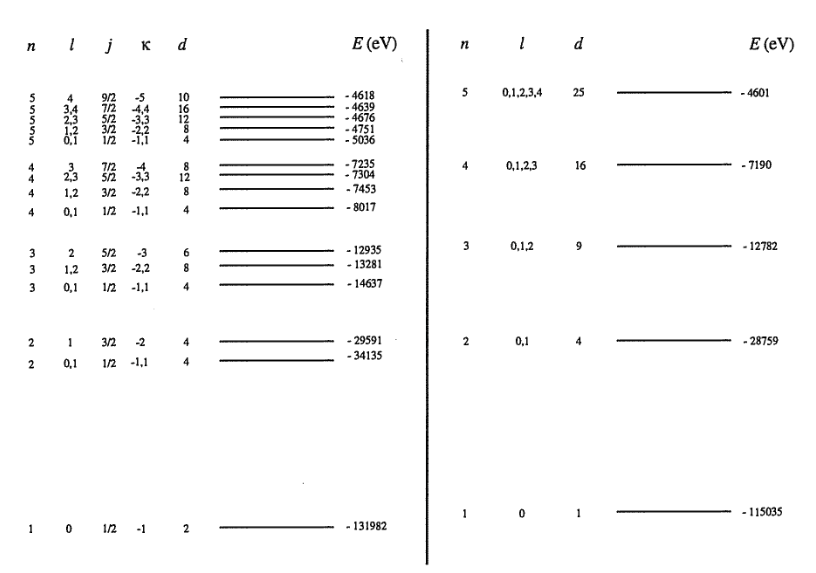
\includegraphics[width=\textwidth,height=\textheight,keepaspectratio]{Figures/relativistic.png}
\end{figure}
\end{frame}

\begin{frame}
 \begin{itemize}
  \item Los efectos relativistas ser\'an m\'as notorios con n\'umero cu\'antico principal peque\~no.
    \vspace{3mm}
  \item Para un orbital dado, el corrimiento relativista es m\'as grande entre m\'as grande sea Z. Corroborado por c\'alculos m\'as sofisticados y el experimento. \\
  Ejemplo: desdoblamiento de los niveles $2p$ entre $j=l+1/2, \kappa = -2$ y $j=l-1/2, \kappa = 1$
  \begin{enumerate}
   \item Al (Z=13) $\implies \Delta E \approx 1.3 eV$
   \item Fe (Z=26) $\implies \Delta E \approx 21 eV$
   \item U (Z=92) $\implies \Delta E \approx 4500 eV$
  \end{enumerate}
  \vspace{3mm}
  \item Estos desdoblamientos salen naturalmente de la teor\'ia relativista, mientras que en el caso no relativista se debe introducir emp\'iricamente el acoplamiento spin-\'orbita al Hamiltoniano.

 
  \end{itemize}

\end{frame}

\begin{frame}{Conclusiones}

\begin{itemize}
 \item  Se predijo correctamente los niveles de energ\'ia del \'atomo de Hidr\'ogeno (\'atomo de 1 electr\'on)
  \vspace{1mm}
 \item Concuerda con las l\'ineas de emisi\'on observadas experimentalmente, confirmando as\'i que el \'atomo de Hidr\'ogeno tiene sp\'in $1/2$.
 \vspace{1mm}
 \item Se formaliza la introducci\'on emp\'irica que hizo Pauli del spin.
 \vspace{1mm}
 \item Advertencia: el espectro predicho no es absolutamente exacto. Ejemplo: $2s^{1/2}  $ y $2p^{1/2}$ no est\'an realmente degenerados. La interacci\'on del electr\'on con el el momento magn\'etico del n\'ucleo (estructura hiperfina) y el efecto Lamb levantan la degeneraci\'on.
\end{itemize}

\end{frame}

\end{document}
